\section{Availability}

Availability measures the delivery of correct service as a fraction of the time that the system is ready to provide a service. 
\\
%A system is an entity that interacts with other entities, which constitute the environment of the system and
%can be other systems, humans or the physical world \cite{1335465}. Fundamental properties of communication systems
%are \textit{functionality, performance, security and dependability}. 
The services provided by the system through it's service interface to the user(s) 
is described by the functional specification. Whenever the provided service
deviates from correct service a system failure, called \textit{outage} or \textit{downtime}\footnote{in contrast, \textit{uptime} does not guarantee correct
service - for example, a server can be 'up' but unreachable} occurs. A failure is defined to be caused originally by a fault inside the system, which may be 
dormant. Under special conditions, the fault \textit{may} become apparent and lead to an error. Faults can be categorized into random and systematic faults:
random faults are unpredictable and concern hardware: for example, because of aging, a memory cell can be damaged, but the fault may be hidden because the cell
is not used. Software and design faults belong to systematic faults. Similar to the damaged memory cell, a software bug may only 
trigger an error under special inputs. In both cases, the error then causes a deviation from the required operation of the system or a subsystem. Finally, the 
error can cause a failure if the system fails to provide the correct service:
\begin{align*}
 fault \rightarrow error \rightarrow failure
\end{align*}
Availability is measured subjectively from the system user's point of view.
While an optimal system may have availability of 1, this value is only of theoretical value because random faults can not be ruled out. Therefor,
system failures are inevitable, and availability is often given in \textit{x-9s}\footnote{read 'one-nine', 'two-nines', ...} notation, denoting the 
number of nines in the time fraction the system delivers correct service, as shown in table \ref{table:x-9}.
The availability may be asserted by the provider of the system to the customer by an
\gls{sla} - if the \gls{sla} is violated, the provider may be fined.
\begin{figure}
    \centering
    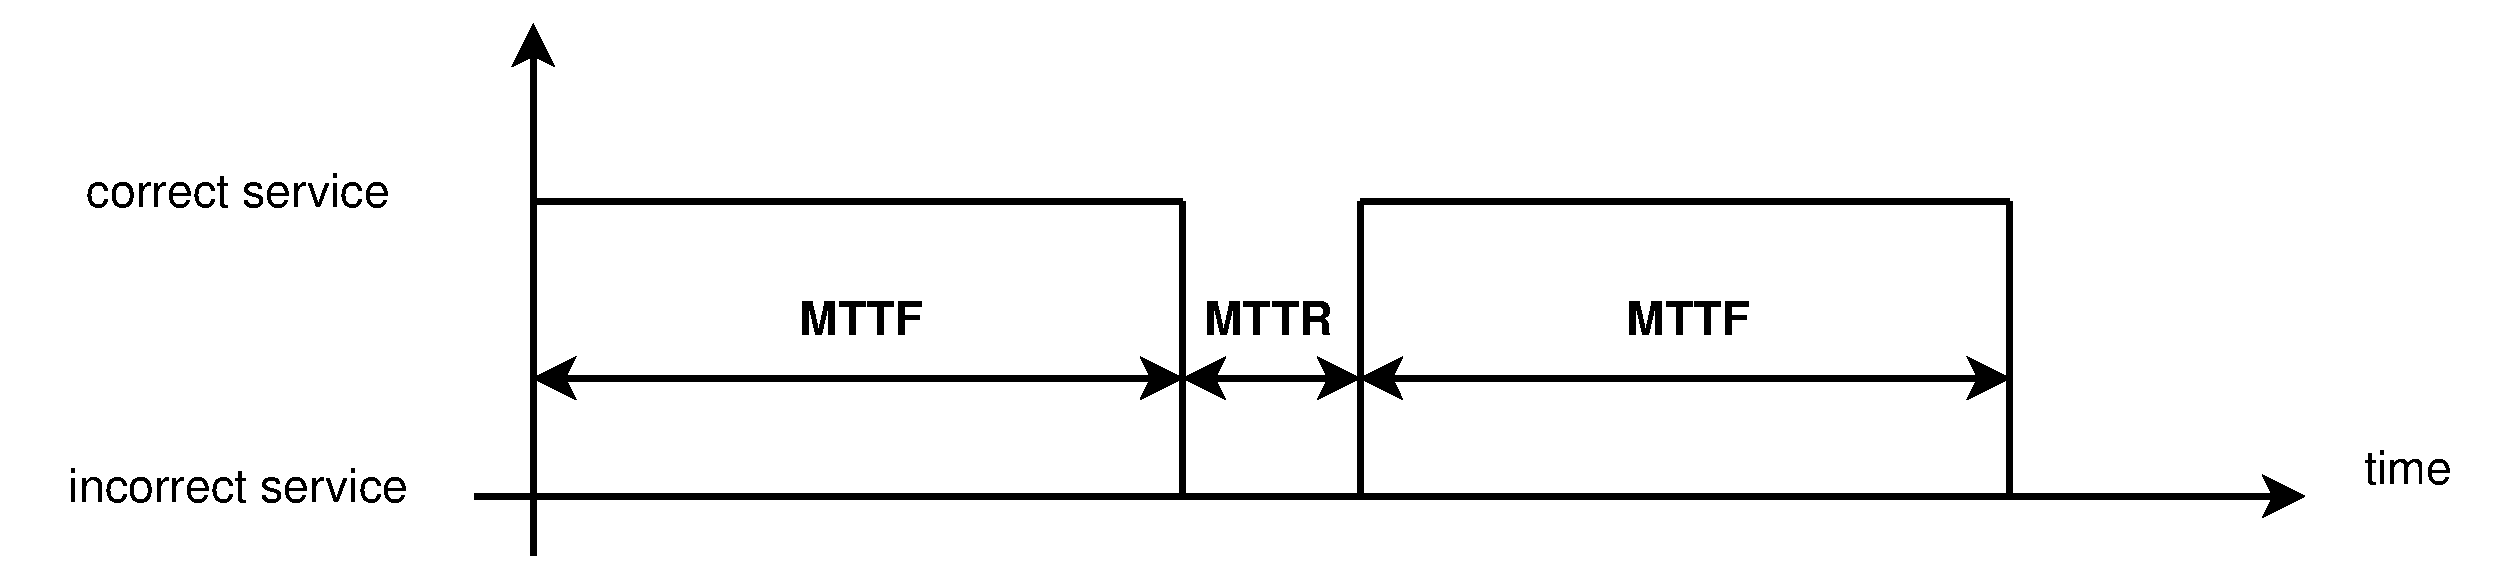
\includegraphics[width=1\textwidth]{figures/availability}
    \caption{Relationship between \gls{mttf} and \gls{mttr}}
    \label{fig:relmttfmttr}
\end{figure}
\begin{center}
\begin{tabular}{ c | c c  }
 \label{table:x-9}
  x & $P_{availability}$ & failure duration per year \\ \hline
  1 & 90,0000    & ~ 36 days \\
  2 & 99,0000    & ~ 3,5 days  \\
  3 & 99,9000    & ~ 9 hours \\
  4 & 99,9900    & ~ 1 hour \\
  5 & 99,9990    & ~ 5 minutes \\
  6 & 99,9999    & ~ 31 seconds \\ 
  
\end{tabular}
\end{center}
For a system with 6-9 availability, this would mean that the system provider assures that the system will be unavailable not more than about 31 seconds over a
whole year.
\\
\\
Availability is important simply because unavailable systems cause costs. Because of the relation of availability to reliability and the maintainability
of the system, as shown in equation \ref{EQUavailability} and figure \ref{fig:relmttfmttr}, two options to improve availability exist: either increasing
the \gls{mttf} (i.e. increasing reliability) or decreasing \gls{mttr}.
%An informal definition of a dependable system is a system which delivers a service that can be justifiable trusted. More formally,
%dependability consists of the following attributes:
%\textit{Availability}, which means that the system is ready for correct service, \textit{reliability}, the continuity of correct service,
%\textit{safety}, i.e. the avoidance of catastrophic consequences \textit{integrity}, s.t. the system cannot be modified in an unwanted manner
%and \textit{maintainability}, so that the system can be repaired in the case of a failure.
%In case of a secure system, another important property is \textit{confidentiality}, which means that no information is disclosed to unauthorized 
%entities.
\begin{align}\label{EQUavailability}
 P_{Availability} = \frac{t_{correct\ service}}{t_{total}} =  \frac{{\gls{mttf}}}{\gls{mttf}+\gls{mttr}}
\end{align}
Reliability measures the probability that the service will work as expected until time $t$:
\begin{align}\label{expFailLaw}
 R(t) = e^{-\lambda(t-t_0)}
\end{align}
\ref{expFailLaw} is known as the \textit{exponential failure law}, $\lambda$ denotes the failures per hour, it's inverse $\frac{1}{\lambda}$ is
called \gls{mttf}. Reliability can also be expressed in terms of \textit{un}reliability, denoted $Q(t)$:
\begin{align}
 Q(t) = 1 - R(t)
\end{align}
Maintainability measures the time that is needed to repair a system, with $\mu$ denoting the repair rate and $\frac{1}{\mu}$ called \gls{mttr}.
\\
\\
Every system will most likely consist of different and distinct components, each with it's own reliability and failure rates. The final system
will possess an overall reliability, determining it's availability. To model the resulting system, the components will be put together in a mixture of
serial and parallel systems.
\begin{figure}
    \centering
    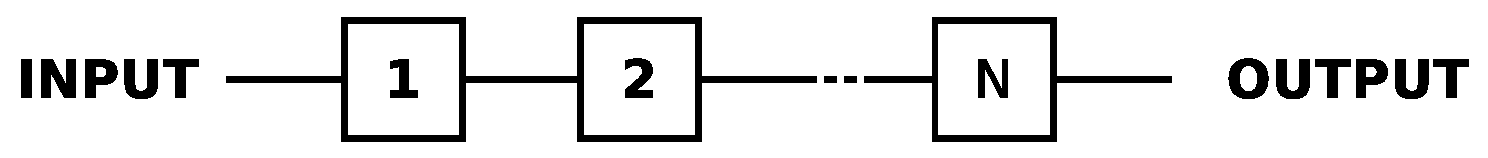
\includegraphics[width=0.8\textwidth]{figures/seriesSystem.eps}
    \caption{Model of a series system}
    \label{fig:serSys}
\end{figure}
For example, if all $i$ components, ranging from $1$ to $N$, are necessary to work correctly for the overall system to deliver correct service, this can be modeled as
a series system, see figure \ref{fig:serSys}. This does not mean that the components are necessarily connected in a serial way, it just stresses that failure
of one single components breaks the whole system. System's reliability then equals the product of all component's reliabilities:
\begin{align}
R_{system}(t) = \prod_{i=1}^{N} R_{i}(t) 
\end{align}
In contrast, a system containing redundant components, failure of one such component must not produce an outage of the overall system. This can be modeled as
a parallel system \ref{fig:parallelSys}. Here, the overall reliability can be calculated as given in \ref{parallelSysEqu}.
\begin{figure}
    \centering
    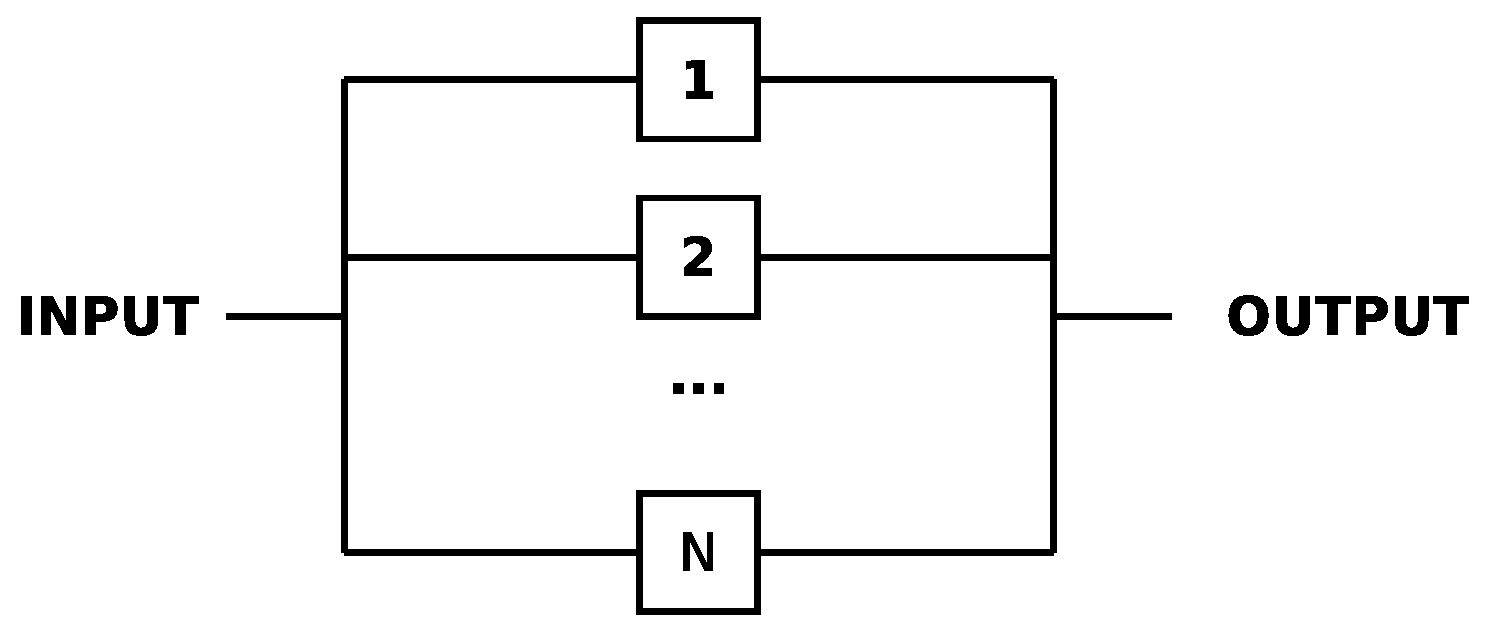
\includegraphics[width=0.8\textwidth]{figures/parallelSys.eps}
    \caption{Model of a parallel system}
    \label{fig:parallelSys}
\end{figure}

\begin{align}\label{parallelSysEqu}
 R(t)_{system} = 1 - \prod_{i=1}^{N} 1- R_{i}(t) = 1 - \prod_{i=1}^{N} Q_{i}(t)
\end{align}
Mixed systems, containing paralell and series system, can be calculated by iteratively condensing serial- or parallel subsystems into single components,
as shown in figure \ref{fig:mixedSys}.
\begin{figure}
    \centering
    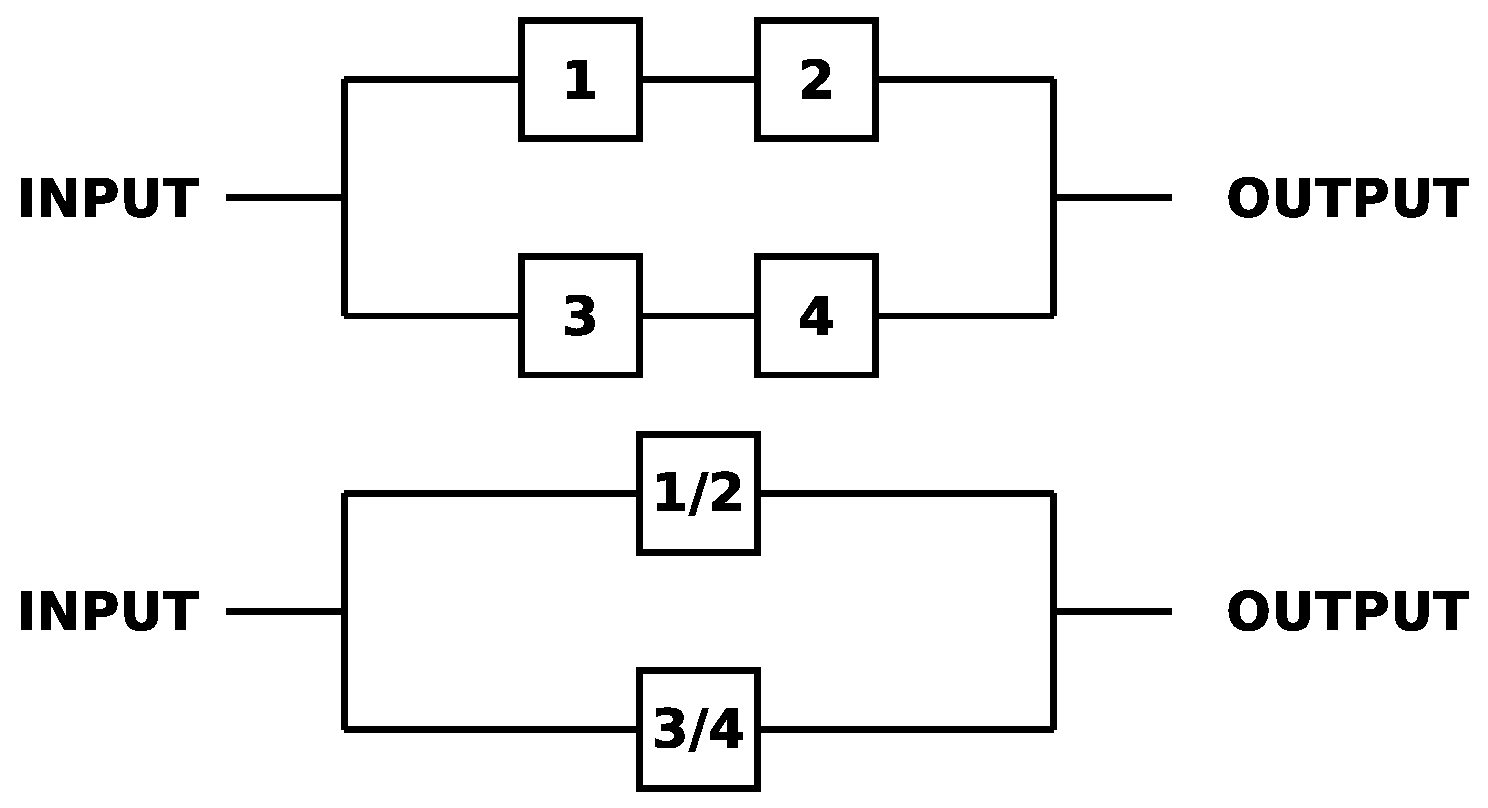
\includegraphics[width=0.8\textwidth]{figures/mixedSys.eps}
    \caption{Condensing a mixed system}
    \label{fig:mixedSys}
\end{figure}
\\
\\
\gls{ha} characterizes a system that is designed in a way to avoid outages, or in case of a failure that can be repaired in shortest possible time. 
The level of the needed availability depends on the environment of the system and must be weighted against the additional costs, introduced by improving availability.
Therefor, no hard definition for \gls{ha} can be given - it is a design goal and depends on the context. Availability requirements will most certainly be higher
for systems in safety-critical requirements. A safety-critical system must not fail, otherwise endangering human lives or 
causing substantial economic loss or environmental damage \cite{1007998}.
On the other side, systems that will produce only minor costs when not operating correctly
will probably have to meet less stringent availability levels.
\\
For example, our society heavily depends on electric power supply, an outage
is nearly unacceptable. On the other side, it is impossible to guarantee 100\% availability, so \textit{if} a power outage occurs, the system must be fixed as soon as
possible to restore correct service, otherwise risking human lives. On the contrary, a booking system will obviously result in financial losses for the company 
if not working, but no more serious consequences are to be assumed.
\\
\\
This work's focus lies on security-critical systems, increasing availability of KNX networks, but restricting it's
deployment to environments without safety-critical needs. Thus, safety criticality is neglected here because of it's most stringent demands, as needed in
avionics or weapons systems.
The difference between safety-critical and security-critical systems can be given as follows \cite{5784222}: safety means that software must not be harm the 
world (i.e. containment), while security means that the world must not harm software (i.e. protection).

\section{Failure Avoidance}

Different strategies exist to handle faults, thus trying to avoid that a fault propagates through the system and finally leads to a system failure.
These strategies are introduced in the next section.

\subsection{Fault Removal}
Fault removal tries to identify faults by testing the system before its deployment. 
\\
Therefor, the system is exposed to test cases, which ideally would cover all possible internal states. Whenever a failure occurs, the erroneous state is identified, the
underlying fault is removed and a new testing cycle begins.
\\
A problem about this approach is the huge test space that for even simple systems would be required to iterate through. Therefor, the method suffers from the very
fundamental dilemma that testing never can proof that a system is fault free.
\subsection{Fault Avoidance}
Fault avoidance aims at producing a system which is fault-free
per design and is applied at the design stage of the system. Despite the methods for achieving fault avoidance can be applied in the domain of sofware and hardware,
they can not guard against transient hardware faults occurring after the system is deployed.
\\
Fault avoidance is based on two distinct processing steps: validation and verification. Validation is used to to show that the specification, which is
the basis of system implementation, matches the real world within reasonable borders. This is necessary because every human built system uses an abstraction
of the real world, thus simplifying the model.
\\
In contrast, verification assures that the system indeed matches the specification. In other words, validation tries to answer if the correct system was built,
while verification is concerned about to build the system correctly.
\\
\\
Formal methods can be be utilized for verification if the system model is available in a formal language. The formal properties of the specification can then be 
checked automatically against a finite-state model of the system, a method called \textit{model checking}.
\\
While automatic validation can proof that the resulting system is correct in regard to the specification, a big problem here is to obtain the formal properties
out of an informal specification.
\\
\\
\\
Obviously, both fault removal as well as fault avoidance cannot handle deliberately introduced faults, caused by an active adversary.
Additionally, they cannot deal with hardware errors -  therefor it is argued that fault tolerance is the only practical way to guarantee availability
in a hostile environment (i.e. an environment where active attackers are assumed to exist and therefor \gls{dos} attacks cannot be ruled out), as well as to
protect against random hardware errors.
\\
Consequently, the proposed solution will be based on fault tolerance to achieve \gls{ha}, which will be examined more detailed.
 
\subsection{Fault tolerance}
Fault tolerance tries to ensure correct service despite the occurrence of faults and is achieved through error detection and subsequent system recovery.
To enable error detection, redundancy is added to a system and thereby the 
system's complexity is increased. This can be achieved booth in the domain of hardware and software. 
\\
The basis of the design of fault tolerant systems is the definition of a \textit{fault hypothesis}, stating which faults must be tolerable by the system, thus
dividing the fault state into normal faults and rare faults (i.e. faults not covered by the fault hypothesis). Normal faults can be corrected by the fault-tolerance
mechanism. 

\subsubsection{Fail-silent fault tolerance}
Fault tolerance can be achieved based on \textit{fail-silent} components. A fail-silent component
either works correctly, i.e. outputs correct values, or does not output any values at all \cite{544479}. By duplicating such a module and comparing the
outputs, fault tolerance can be achieved by cutting off the faulty module from the system.
\\
This method is used for example for \gls{raid} based date storage \footnote{although the logic distributing
the data chunks to different devices can be built in hardware or in software, i.e. the operating system, \gls{raid} always relies on redundant disks}.
For \gls{raid} level 1, all data to be stored is duplicated to two independent disks. In case a hardware failure of one drive is detected, the data can be accessed
from the second drive. This method does obviously not work if booth drives seem operable, but one drive outputs bogus data, i.e. it is not acting fail-silent.
To handle this situation, higher redundancy levels are needed, as implemented for example in \gls{tmr}. 

\subsubsection{\gls{tmr}}
A \gls{tmr} system, see figure \ref{fig:tmr}, is composed out of 3 modules or \textit{black boxes}, all performing the same task,	
and one \textit{majoriy organ} $V$, as proposed by Von Neumann \cite{vN56}. The latter element
is also called \textit{voter} because out of it's 3 inputs, it chooses the 'correct' output based on majority voting. As long as at least 2 black boxes do not
fail, the system can provide correct service. If it is assumed that the voting element has perfect reliability = 1 and all black boxes $M$ are independent from
each other and have reliability $R_M$, the overall, time-invariant system's reliability is given in \ref{tmrEq} \cite{Lyons:1962:UTR:1661979.1661984} and plotted in graph \ref{fig:tmrGrp}
\begin{align}\label{tmrEq}
 R_{system} = {R_M}^3 + 3{R_M}^2(1-R_M) = 3{R_M}^2 - 2{R_M}^3
\end{align}
\begin{figure}
    \centering
    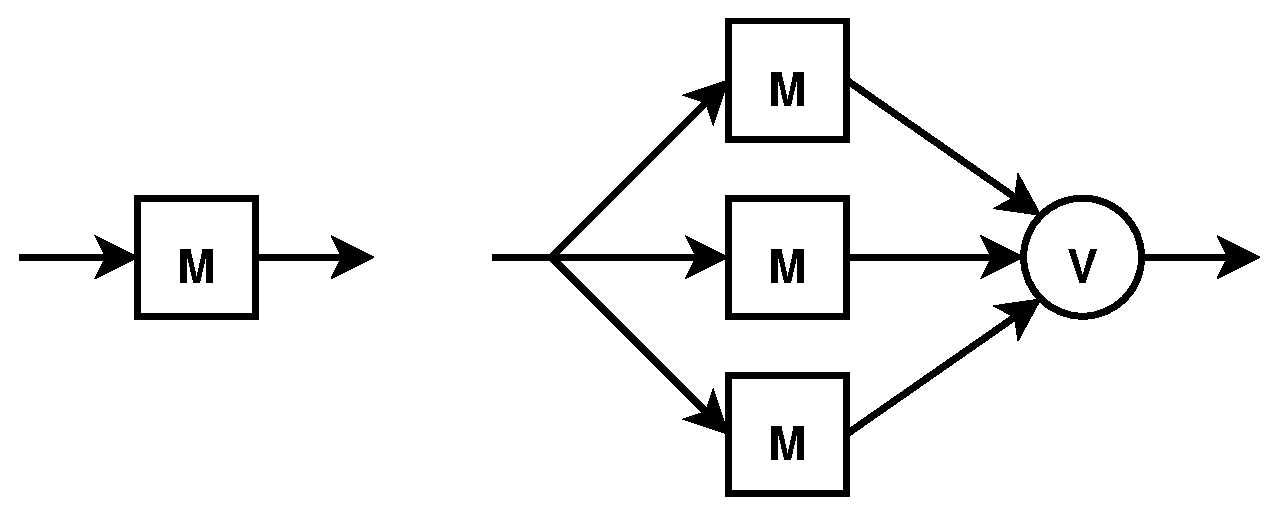
\includegraphics[width=0.8\textwidth]{figures/tmr.eps}
    \caption{Non-redundant operation vs. \gls{tmr}}
    \label{fig:tmr}
\end{figure}
\begin{figure}
    \centering
    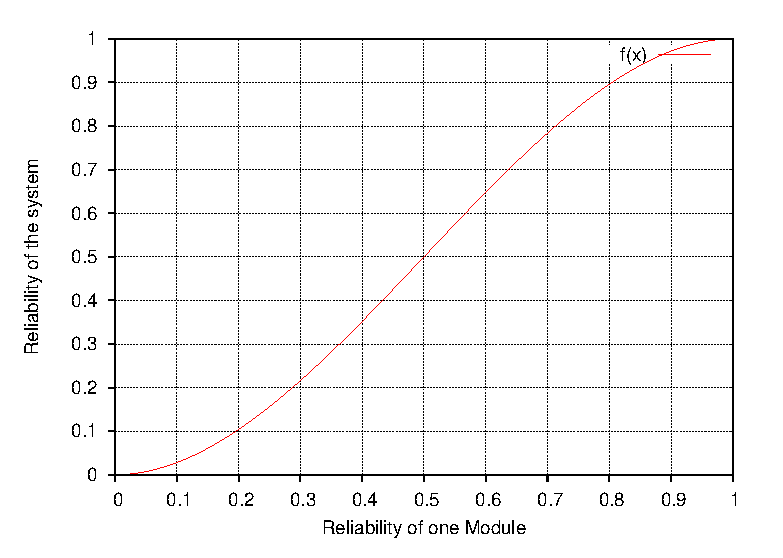
\includegraphics[width=0.8\textwidth]{figures/tmrGraph.eps}
    \caption{Reliability of resulting system}
    \label{fig:tmrGrp}
\end{figure}
It can be seen that if $R_M \leq 0.5$, overall reliability even worses, while for components reliabilities nearly being unit, very high system reliability can
be achieved.
\\
\\
The concept of \gls{tmr} can be generalized to $n$ devices performing
the same operation. In most cases $n$ will be odd, so failure of at least $\frac{n-1}{2}$ modules can be tolerated.

\section{Fault Tolerant Technologies}
In the next sections, communication protocols based on ethernet, satisfying the needs of industrial communication networks, are examined. Beside the need for high availability,
industrial production lines
are sensitive against network disruptions. While, depending on the application domain short interruptions in the range of milliseconds to seconds may be
tolerable, longer outages will force emergency stops or even cause damage.

\subsection{Network redundancy}

Communication networks can be modeled as graphs. A graph, as shown in figure \ref{fig:graph}, is an ordered pair $G=(V,E)$, with $V$ being the set of vertices and $E$
the set of edges, connecting the vertices. For a weighted graph, every edge is associated to a \textit{cost}. 
\\
A \textit{closed walk} or \textit{cycle} exists if a path from one vertex to itself exists, resulting in multiple paths from one node to others.
Such a network posses intrinsic redundancy, a fact that can be exploited to gain fault tolerant systems.
\\
If the graph is undirected, every line determines a bidirectional communication link. 
\\
A spanning tree of graph $G$ is a subgraph $T$, possessing all vertices $V$ but only a subset of the edges $E' \subseteq E$ s.t. all vertices are reachable,
but no loops exists. In the case of a weighted graph, the weight of the spanning tree is the sum of all existing edges.
\begin{figure}[H]
\centering
 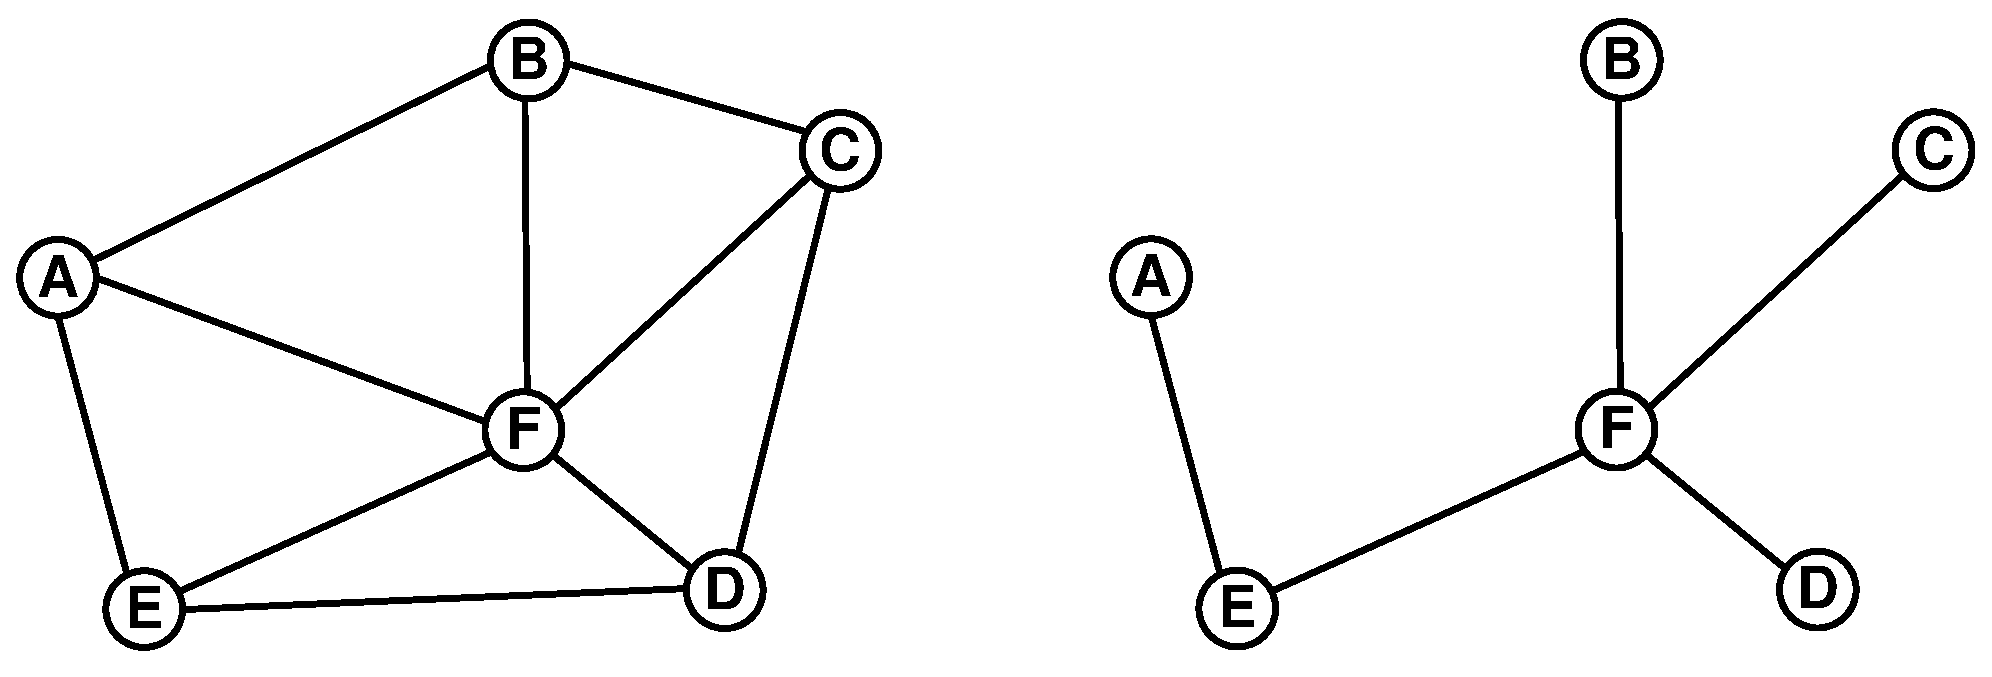
\includegraphics[width=0.8\linewidth]{figures/graph.eps}
 \caption{Undirected graph, spanning tree of the graph}
\label{fig:graph}
\end{figure}

\subsubsection{\gls{stp}}
The widely used \gls{ieee} 802.3 ethernet standard was not designed with high availability in mind.
Nevertheless, it already provided basic fault tolerance mechanisms based on the \gls{ieee} 802.1D \gls{stp}. 
\\
\\
In typical ethernet installations, depending on the network topology different
nodes may be reachable through different paths, i.e. physical loops may exist.
Switches, operating at \gls{osi} layer 2, are responsible for loop detection and
loop prevention and must logically disconnect such loops by blocking the corresponding ports to protect the network,
as required by the ethernet specification, because multicast or broadcast traffic, generated by one of the connected
devices, will be forwarded by all switches on all ports (except the incoming ports), thus flooding the network until no regular communication will be possible any
more.
\\
\begin{figure}[H]
 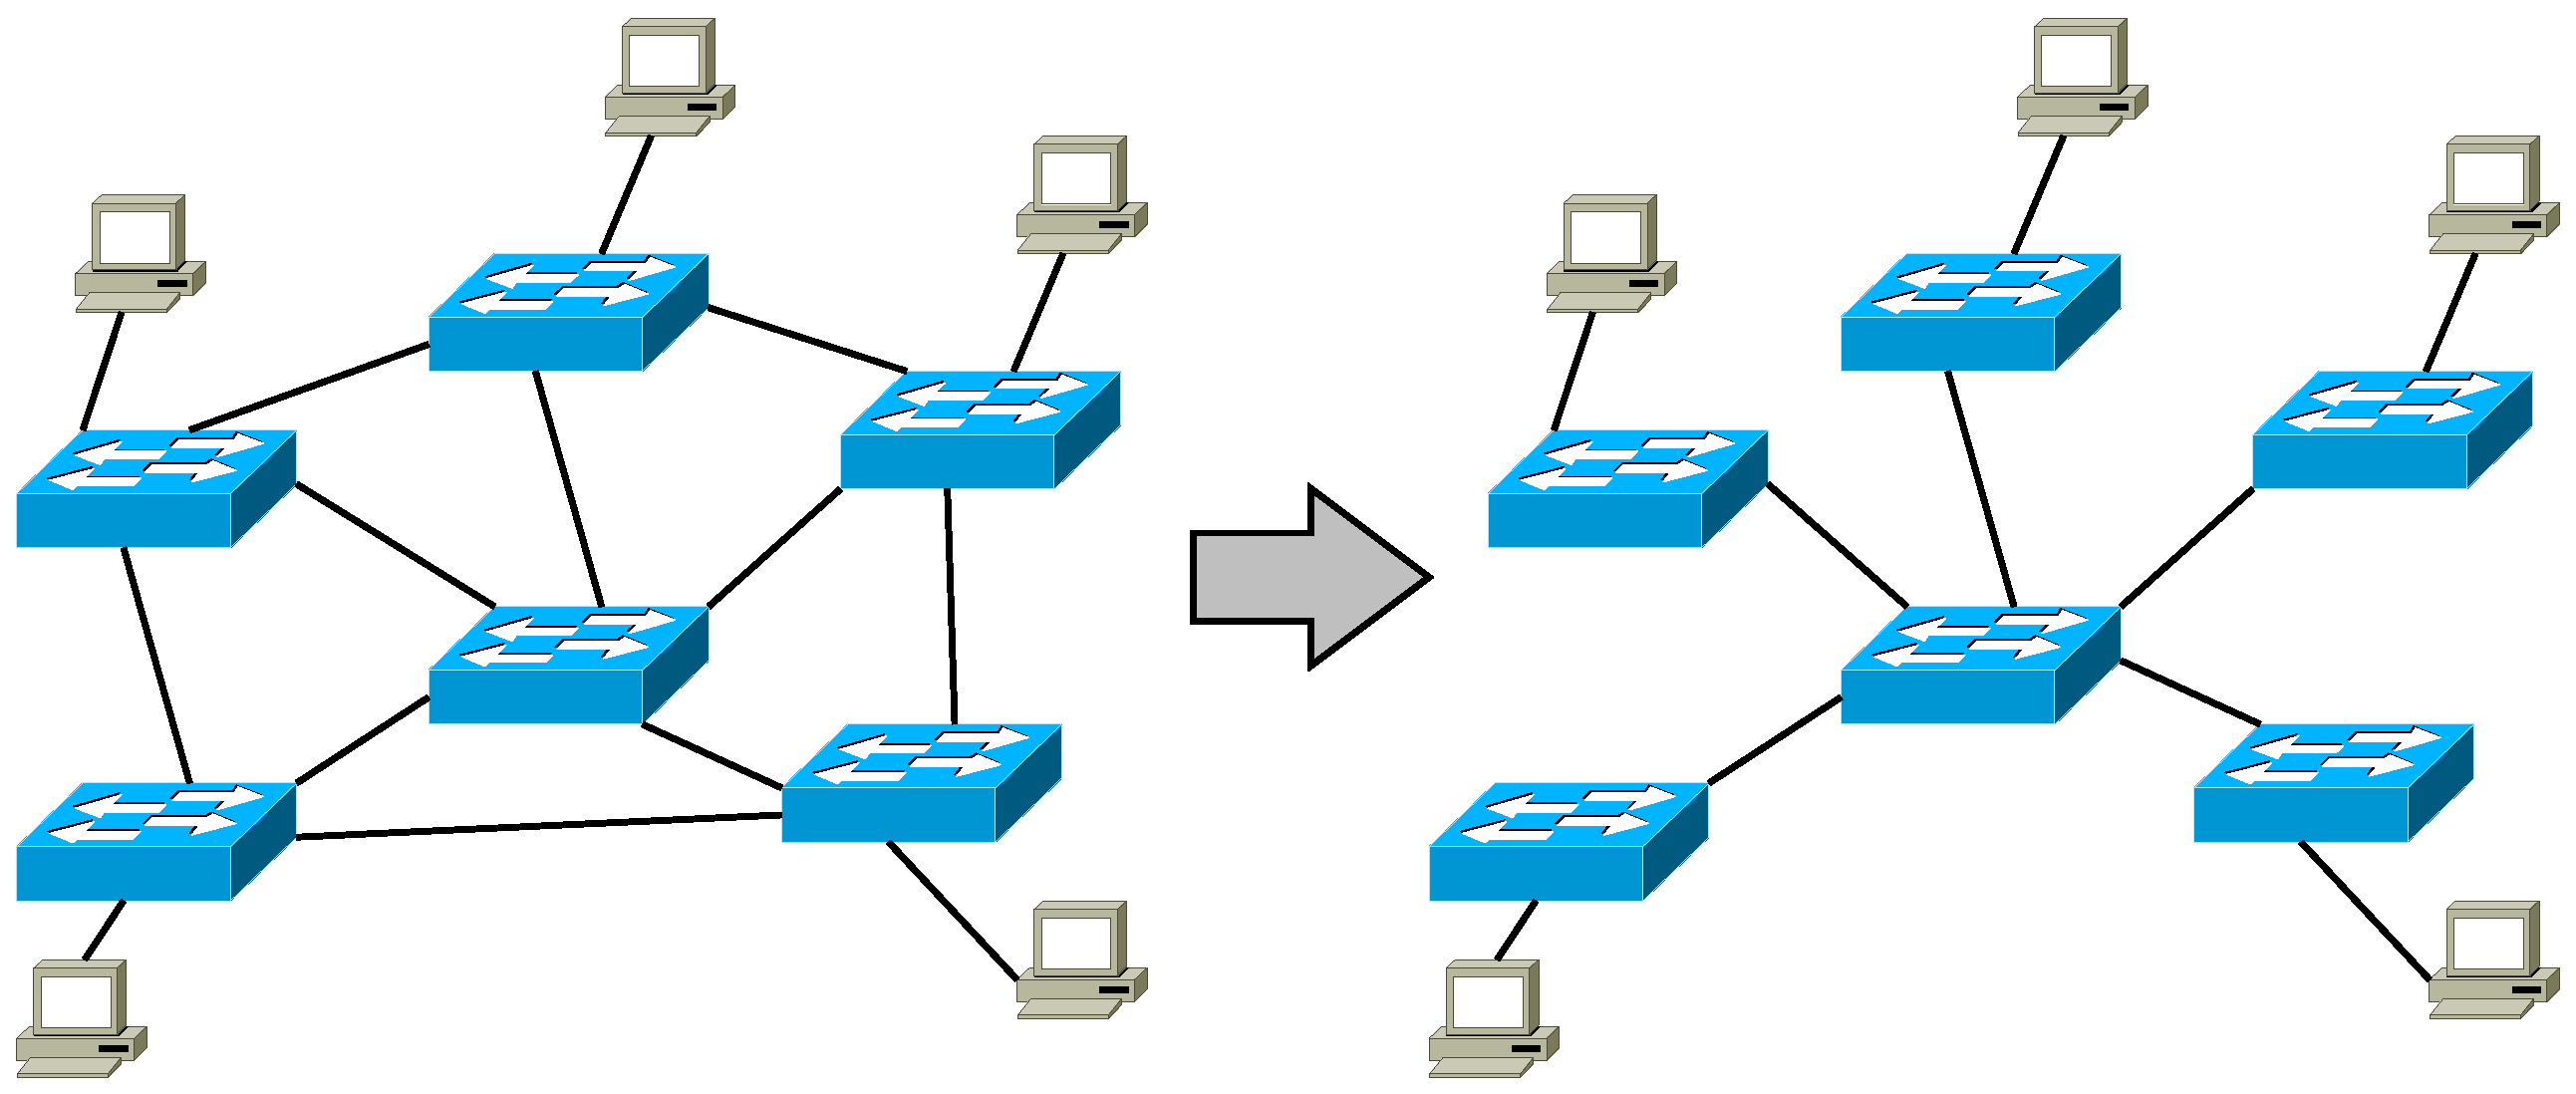
\includegraphics[width=\linewidth]{figures/stp.eps}
 \caption{Protecting ethernet segments from loops with \gls{stp}}
\label{fig:stp1}
\end{figure}
This situation is shown in 
figure \ref{fig:stp1}: on the left side, the physical connections are shown, containing loops. 
\gls{stp} removes
the loops by setting certain interfaces to blocking mode, connected by dotted lines, as shown on the right side of figure \ref{fig:stp1}.
\\
The algorithm works as follows:

\begin{itemize}
 \item The first step of the \gls{stp} algorithm is to nominate one device as root bridge\footnote{the terms \textit{switch} and \textit{bridge} are used synonymously,
with the major difference that switches can break network segments into multiple subsegments through \glspl{vlan}}. This can be done manually by the network administrator,
or dynamically through the exchange of packages containing a priority. All switches will agree on lowest priority device as root bridge, additionally using the unique
hardware \gls{mac} address if collisions occur. The root bridge sets all interfaces to forwarding mode. 
 \item Afterwards, every switch determines the path with minimal costs for reaching the root bridge. The cost of every connection can be determined by the link
 speed or configured by the network administrator manually
 \item Finally, all devices except the root bridge set the ports belonging to the minimal-cost path to forward mode. All other ports are set to blocking mode, thus removing
 any loops.
\end{itemize}
If a connection is lost and an ethernet segment is not 
reachable any more, the \gls{stp}, although not primarily designed for that tasks, can be used to handle that fault. Nodes affected by the link-change report
that event to the root bridge, so that the network can be re-configured and a different path can be established, thus re-connecting the unreachable segment
and providing fault tolerance. 
\\
\\
A big drawback of this mechanism is the topology-dependent
time needed for network re-organization. While in simulations delays of millisecond magnitude can be achieved \cite{4447112}, in practice link recovery
can take up to one minute which is not acceptable for many industrial environments. An improvement was achieved with \gls{ieee} 802.1w \gls{rstp} and
a variety of different proprietary protocols, not compatible to each other, but still no sufficient recovery times were achieved \cite{1704183}.

\subsubsection{IEC 62439}

As it turned out that the mechanisms based on \gls{stp} and it's variations were not 
sufficient for many applications, the family of IEC 62439 standards was defined. IEC 62439 introduces a set of ethernet extensions, assuring high availability
and enabling its deployment in industrial applications. Three extensions are introduced below.

\subsubsection{\gls{mrp}}
After IEC 62439-1 specifying basic definitions, the second draft introduced \gls{mrp} which confines network outages to less than 500ms \cite{6145654}.
This is achieved by restricting the valid topologies to ring-only, so all switches are connected to the network by 2 interfaces. All switches beside the ring manager
forward all traffic received, while the ring manager opens the loop logically by setting one of it's interfaces to blocking mode.
In this mode, all packages except management messages are discarded. The ring manager detects a failure by periodically sending test management messages in booth
directions. Additionally every node is able to detect a link failure on it's local ports. It then sets the port to blocking and signals this link failure to the
ring manager which opens his second port by setting it to forward mode and therefore reconnects the unreachable segment.
\\
\gls{mrp} does not rule out package loss in case of a failure, therefor it can be seen as improved \gls{rstp} for ring topologies. 

\begin{figure}[H]
 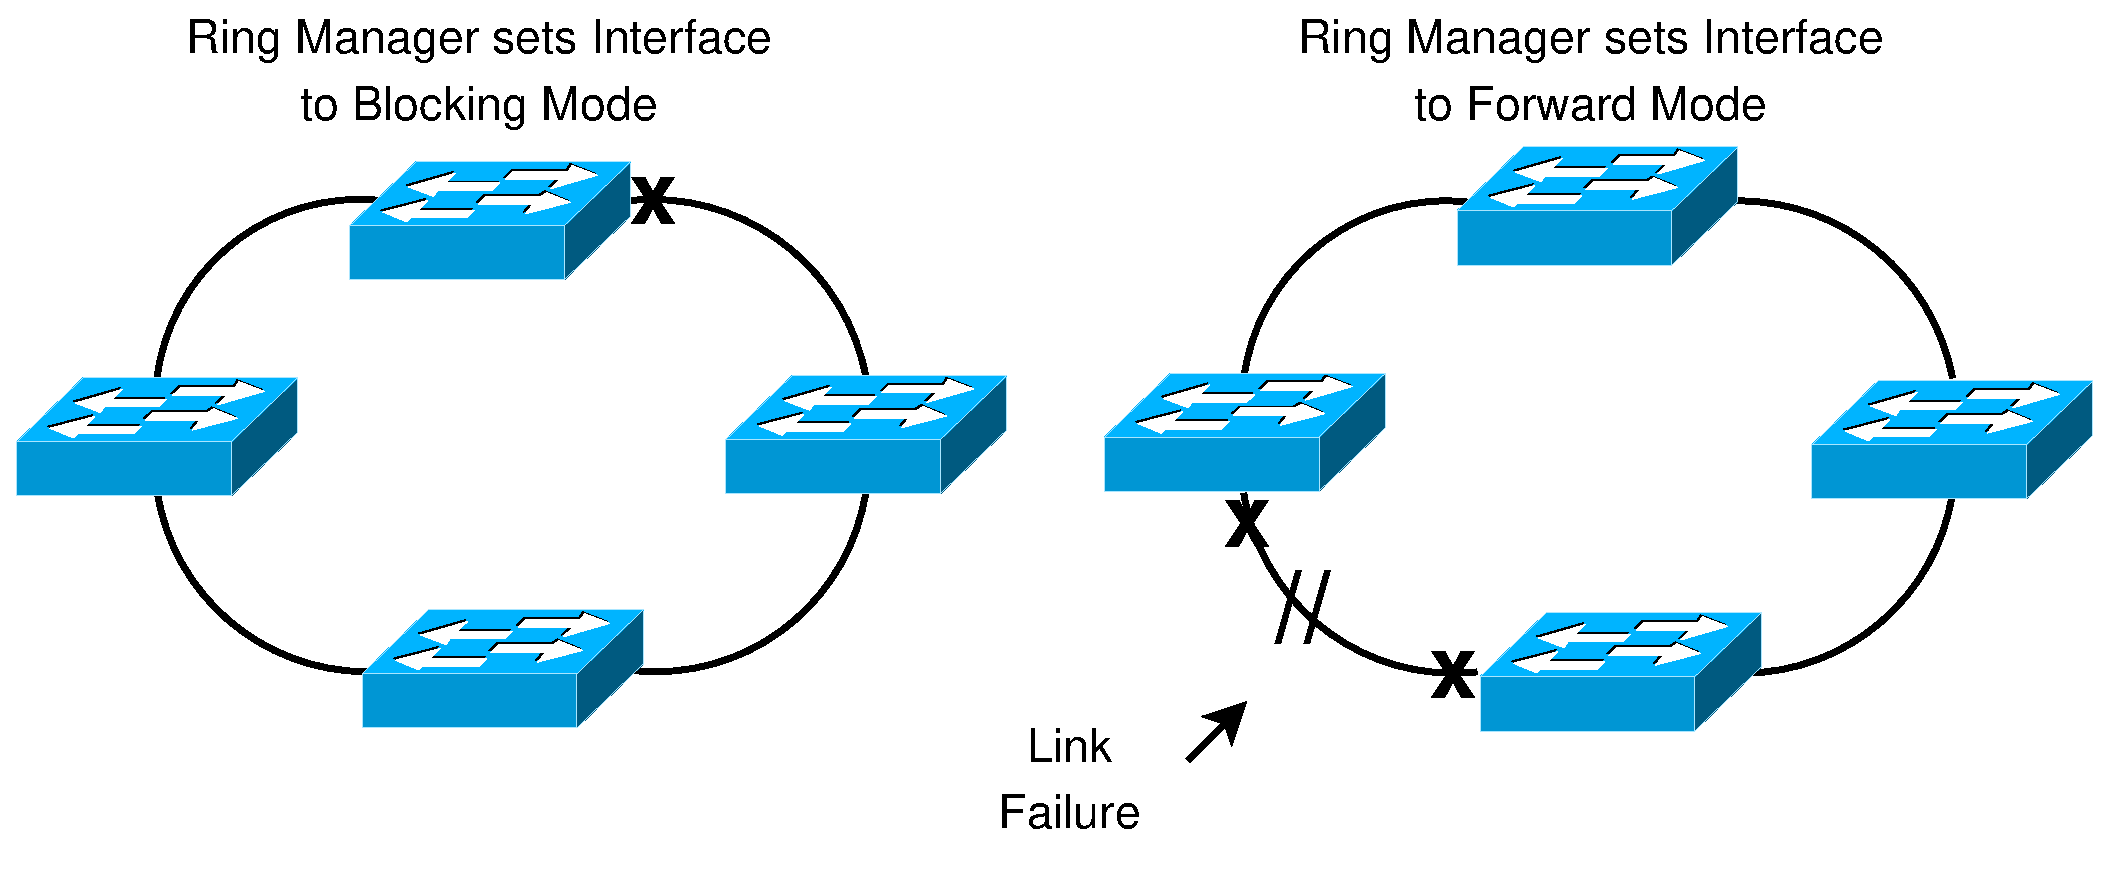
\includegraphics[width=\linewidth]{figures/MRP2.eps}
 \caption{MRP fault tolerance}
\label{fig:mrp1}
\end{figure}


\subsubsection{\gls{prp}}
In 2010, IEC 62439-3 defined a first version of {\gls{prp}} and \gls{hsr}, booth suitable for hard real-time
systems \footnote{hard real-time characterizes a system where missing of a dead line may result in a catastrophic event} \cite{4416946}.
\\
In 2012, IEC 62439-3 was revised, defining new versions of \gls{prp} and \gls{hsr}. The basic ideas behind booth protocols remained
unchanged, so the latest versions are described below.
\\
\\
\gls{prp} can tolerate a link fault without package loss by utilizing two redundant and independent \glspl{lan}.
Nodes needing high availability, called \gls{danp}, are connected to both networks by two interfaces, sharing the same \gls{mac} and \gls{ip} addresses.
Additionally, standard ethernet devices called \gls{san} can be connected to only one network, enabling communication with devices on the same \gls{lan} only.
An example of such a network is shown in figure \ref{fig:prp}.
\\
To support redundant connections for \glspl{danp}, a sub-layer on \gls{osi}-layer 2 (i.e. the link layer), called \gls{lre} is defined. 
Upper level data arriving at the \gls{lre} of a \gls{danp} is duplicated and equipped with 6 bytes of control information, containing a 2 byte sequence number,
\gls{lan} number, length information and a static suffix identifying the \gls{lsdu} as \gls{prp} traffic. The sequence number is used for duplicate detection: 
every node uses one global counter $Ctr_{global}$ for outgoing messages, not discriminating the receiver. For every package sent, the sequence number is incremented.
Additionally, every node maintains distinct counter values $Ctr_{source}$ for every unicast source-address it receives messages from, as well as for multicast
and broadcast messages.
\\
On the receiving side the \gls{prp} traffic is detected because of the suffix, duplicates can be discarded by utilizing the sequence number \cite{6699852}.
The standard does not dictate how this must be achieved, it only demands that legitimate packages must not be discarded. Because of the short global outgoing 
sequence number, duplicates may not be detected as such - responsibility for final detection is delegated to upper layers.
%If the received number is higher than the saved one $C_{source}$, the package is forwarded to the upper layer and the received sequence number is saved as $C_{source}$.
%Therefor, the package transmitted over the alternate line (i.e. the delayed package) will contain a sequence number smaller than the number saved for the 
%corresponding source address and can safely be discarded, thus preventing the processing of duplicate frames by the upper level.  
\begin{figure}
    \centering
    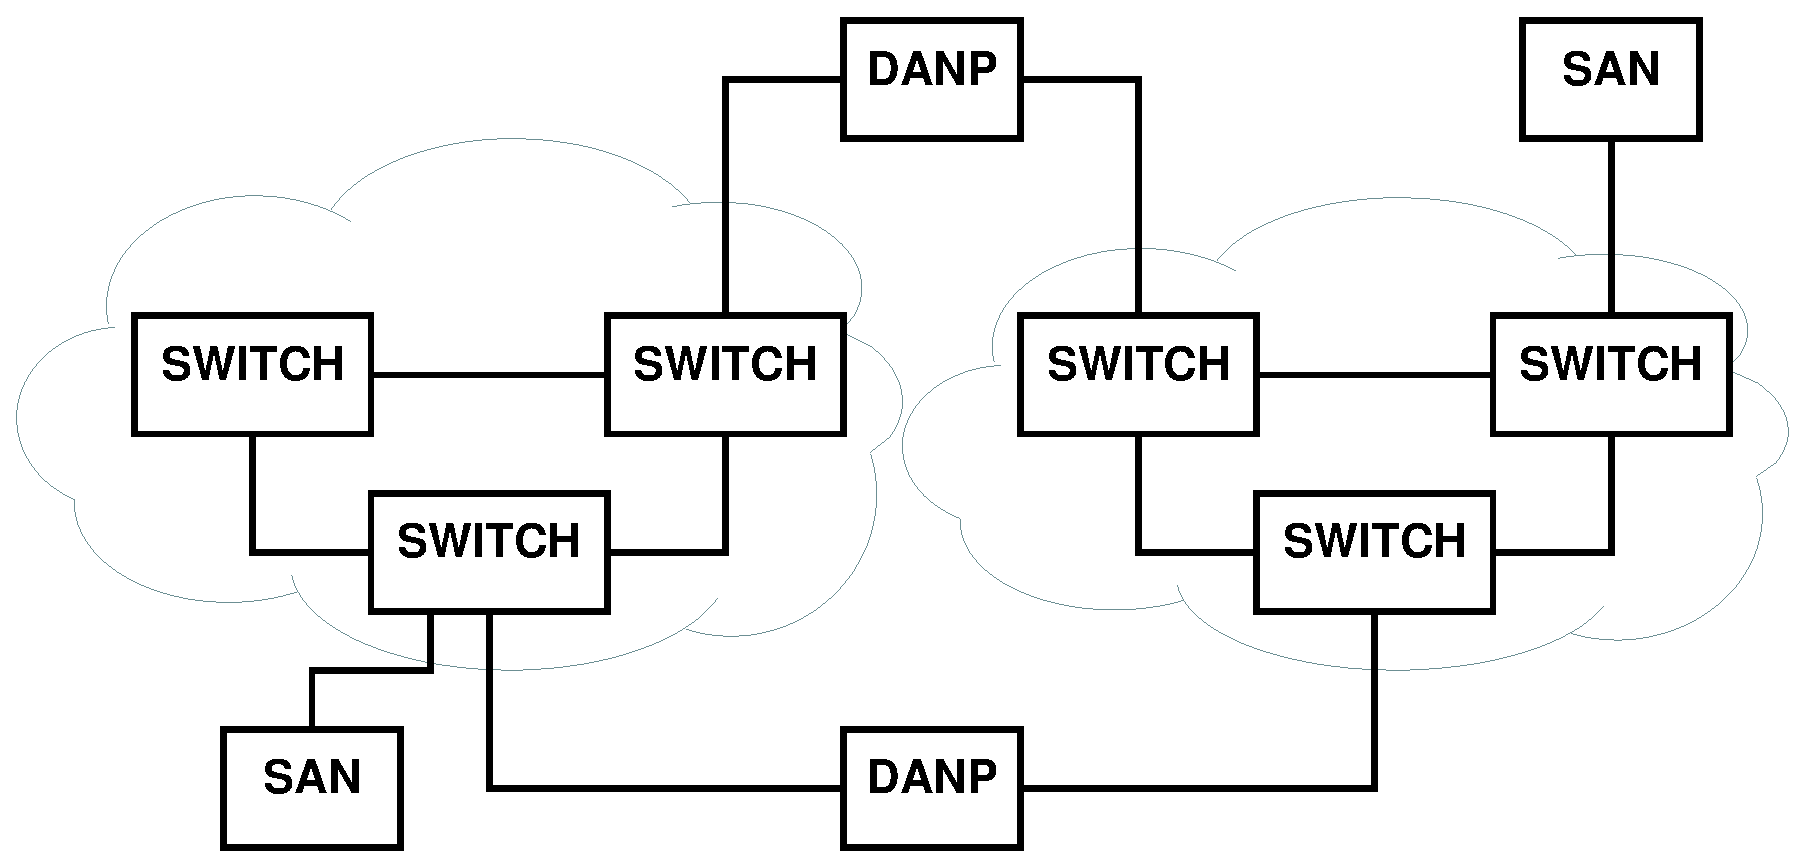
\includegraphics[width=1\textwidth]{figures/prp.eps}
    \caption{\gls{prp} network}
    \label{fig:prp}
\end{figure}

\subsubsection{\gls{hsr}}
\gls{hsr} is based on ring-topology, but it also allows to connect \gls{hsr} and \gls{prp} networks, different \gls{hsr} rings or even to build a ring of rings. 
Every node is connected to the network by two interfaces, duplicating data from upper layers and sending one copy in clockwise, the other copy in counter-clockwise direction,
thus eliminating the need for duplicated networks but wasting about half of the available bandwidth \cite{6174793}. 
\\


